\documentclass[11pt]{report}
\setlength{\topmargin}{-0.3in}
\setlength{\oddsidemargin}{0pt}
\setlength{\evensidemargin}{0pt}
\setlength{\textheight}{46\baselineskip}
\setlength{\textwidth}{47zw}
\setlength\intextsep{0pt}
\setlength\textfloatsep{0pt}
\usepackage[]{graphicx}

\newcommand{\argmax}{\mathop{\rm arg~max}\limits}
\newcommand{\argmin}{\mathop{\rm arg~min}\limits}
\begin{document}

\begin{titlepage}
\title{能動学習: Active Learning}
\date{2017/11/12}
\author{木村 正成}
\maketitle
\thispagestyle{empty}
\end{titlepage}

\tableofcontents
\clearpage

\section{Introduction}

能動学習は,「もし学習アルゴリズムが学習データ全体の中から任意のデータを選択することができる場合,適切な選択によって得られる学習器の性能は向上する」という仮説に基づいている.
例えば一般的な教師あり学習手法では,何百・何千,もしくはそれ以上の大量のラベル付きインスタンスによって学習を行う.
しかし,現実世界の多くの教師あり学習タスクにおいては,ラベル付きインスタンスの入手は非常に困難であったり時間的・費用的コストが必要であったりする場合が多い.

能動学習では,ラベル無しデータの中から次にラベル付けを行うべきデータを選択してオラクル (例えばアノテータやドメインの専門家など)に問い合わせることで,ラベル付与のボトルネックを解消することを目指している.
この手法では,学習者は出来るだけラベル付与のコストを抑えた上で分類性能を向上させることを目指す.
こうした能動学習の研究は,近年のデータ自体は豊富にあるもののラベル付きデータが不足している,もしくはラベル付与のコストが高価であるような機械学習の問題から幅広く研究されている.

\section{能動学習の適用シナリオ}
能動学習者がクエリを問い合わせるシナリオ及びクエリの問い合わせ戦略は複数存在する\cite{settles2010active}.
多くの研究で考慮されている問題設定は以下の3種類に大別される.

\begin{itemize}
    \item Membership Query Synthesis
    \item Stream-based Selective Sampling
    \item Pool-based Sampling
\end{itemize}

\subsection{Membership Query Synthesis}
最初の能動学習のシナリオは,membership queries\cite{angluin1988queries}に基づく学習である.
この設定では,学習者は入力空間内のあらゆるラベル無しインスタンスのラベルを問い合わせることができる.
ここで生成されるクエリは,自然な分布からサンプリングされるものだけではなく,学習者が仮定する任意のインスタンスに対しても問い合わせることができる.

\begin{figure}[h]
\begin{center}
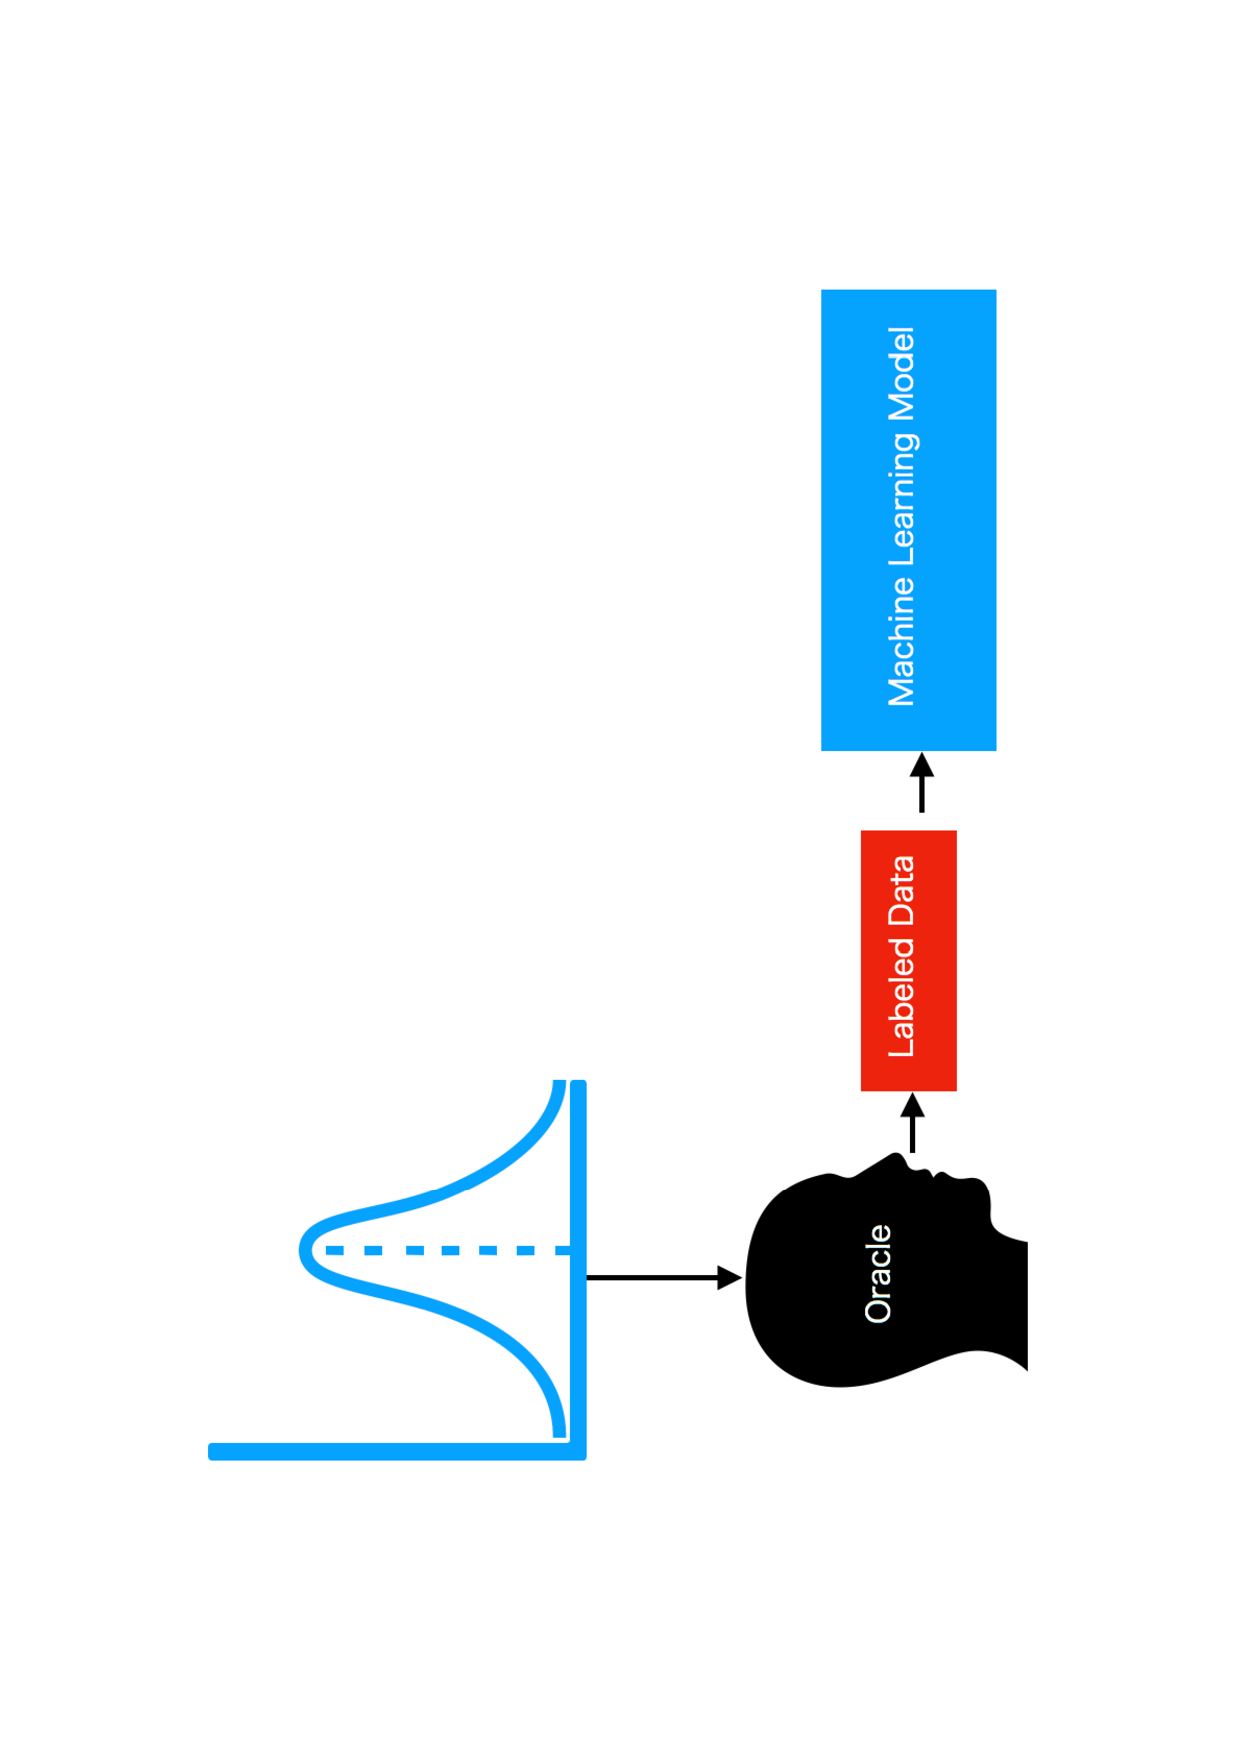
\includegraphics[bb=78 0 500 850, scale=0.4, angle=270]{./images/fig3.pdf}
\vspace{5mm}
\caption{クエリ合成能動学習の例}
\label{fig3}
\end{center}
\end{figure}

こうしたクエリ合成のアプローチは多くの場合で有効である一方で,
オラクルが人手によるアノテータである場合には注意が必要となる\cite{baum1992query}.

\subsection{Stream-based Selective Sampling}
クエリ合成に変わる手法として,selective sampling\cite{atlas1990training}が研究されている.
ここでの主要な仮定として,ラベル無しインスタンスの入手にはコストがかからず,学習者は実際の分布からサンプリングを行なった後にそのインスタンスのラベルを問い合わせるかどうかを決定できる.
こうしたアプローチはストリームベースと呼ばれ,一度に一つのラベル無しデータに対して評価を行う.
入力が一様分布であれば,selective samplingはmembership query学習の様に振る舞う.

\begin{figure}[h]
\begin{center}
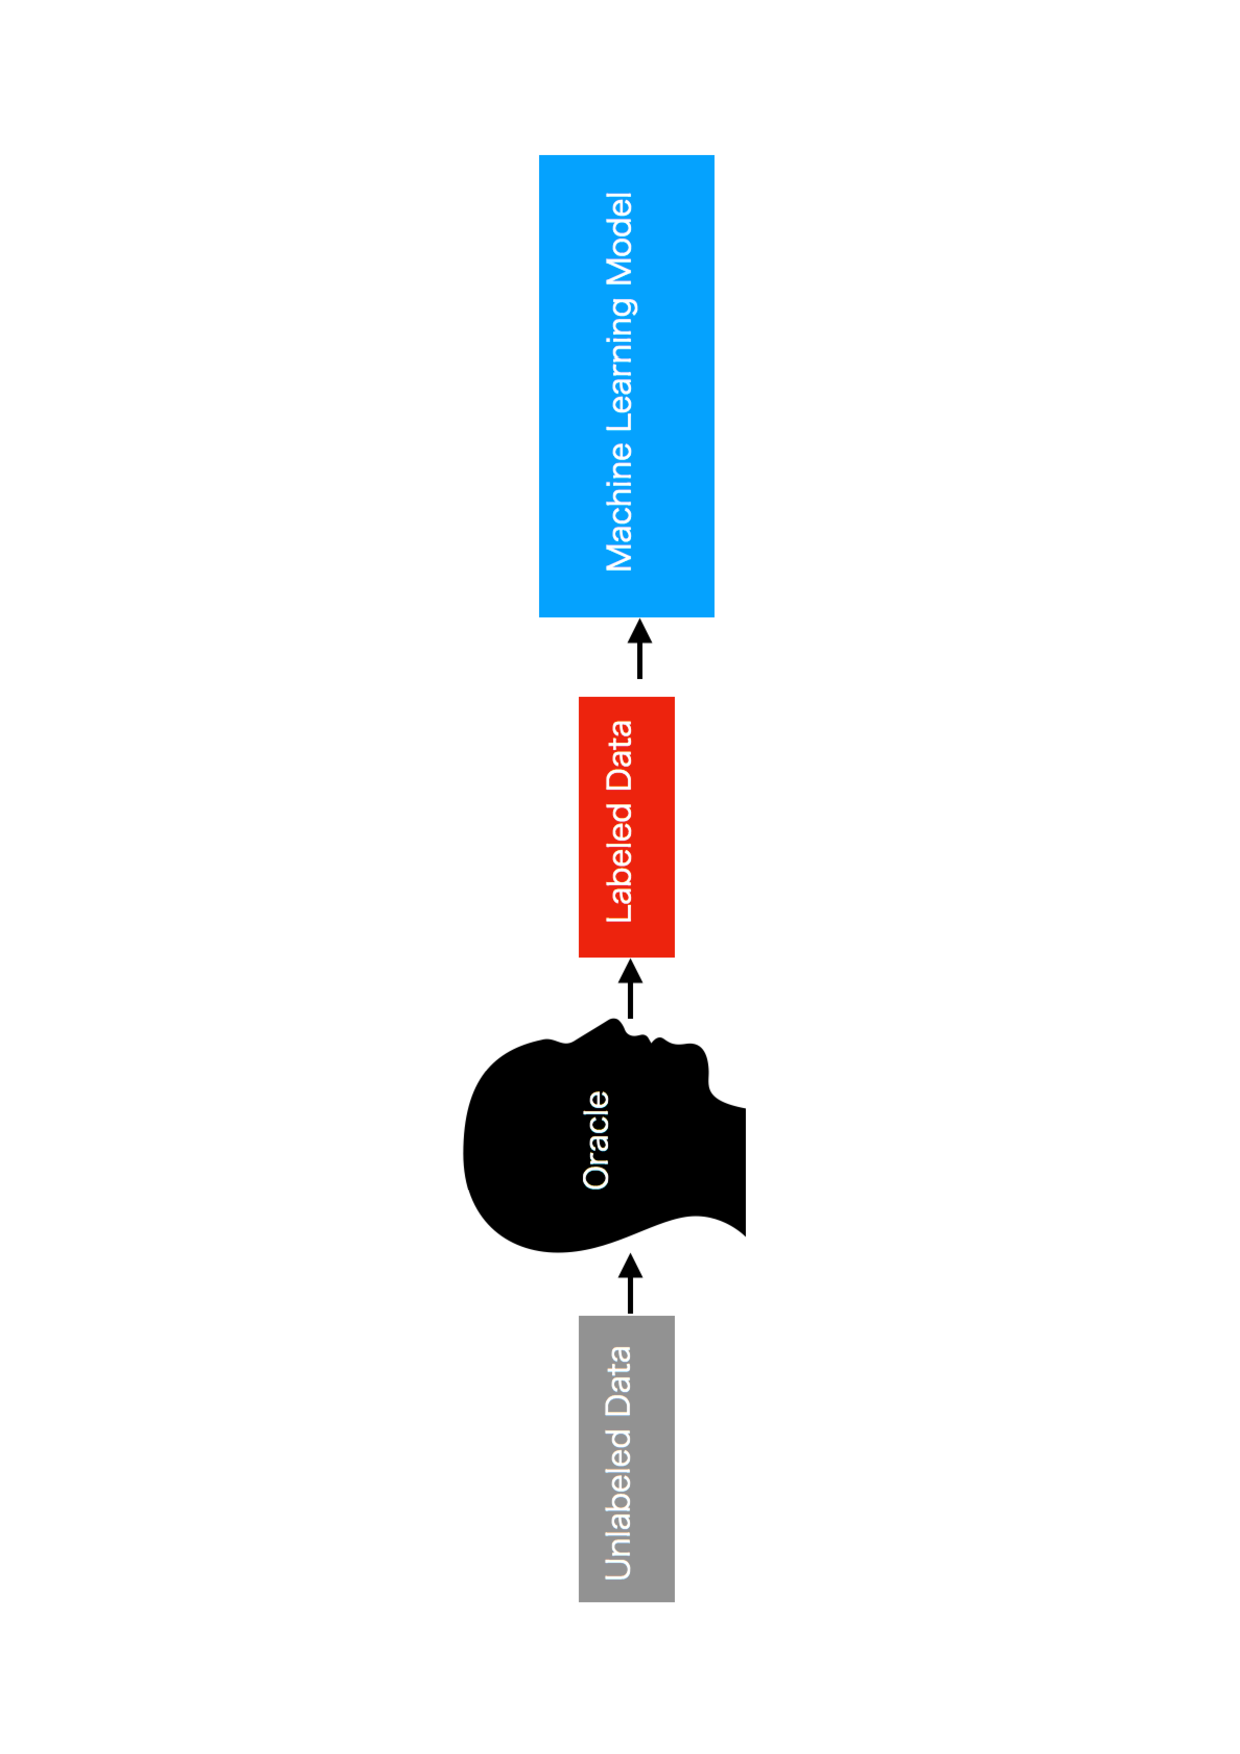
\includegraphics[bb=100 0 350 850, scale=0.4, angle=270]{./images/fig2.pdf}
\vspace{2mm}
\caption{ストリームベース能動学習の例}
\label{fig2}
\end{center}
\end{figure}

あるインスタンスに対してラベルを問い合わせるかどうかの決定は,いくつかの手法によって形式づけられる.
一つの方法として,もっとも情報を持っているようなインスタンスに対してラベルを問い合わせるというものがある\cite{dagan1995committee}.
これを実現するナイーブな方法としては,各インスタンスの情報量の指標に閾値を設けて,それを上回ったインスタンスを選択するなどが考えられる.
また別の手法として,その時点で学習者にとってもっとも曖昧な領域のインスタンスを積極的に選択するというものがある\cite{cohn1994improving}.
これを達成するためには,モデルの出力するクラスの予測確率などを用いるなどが挙げられる.

\subsection{Pool-based Sampling}
多くの現実世界の問題では,巨大なラベル無しデータ集合はあるタイミングで一度に生成される.
このような設定に対応するため,プールベースの能動学習手法が研究されている.Figure\ref{fig1}にプールベース手法の例を示す.

\begin{figure}[h]
\begin{center}
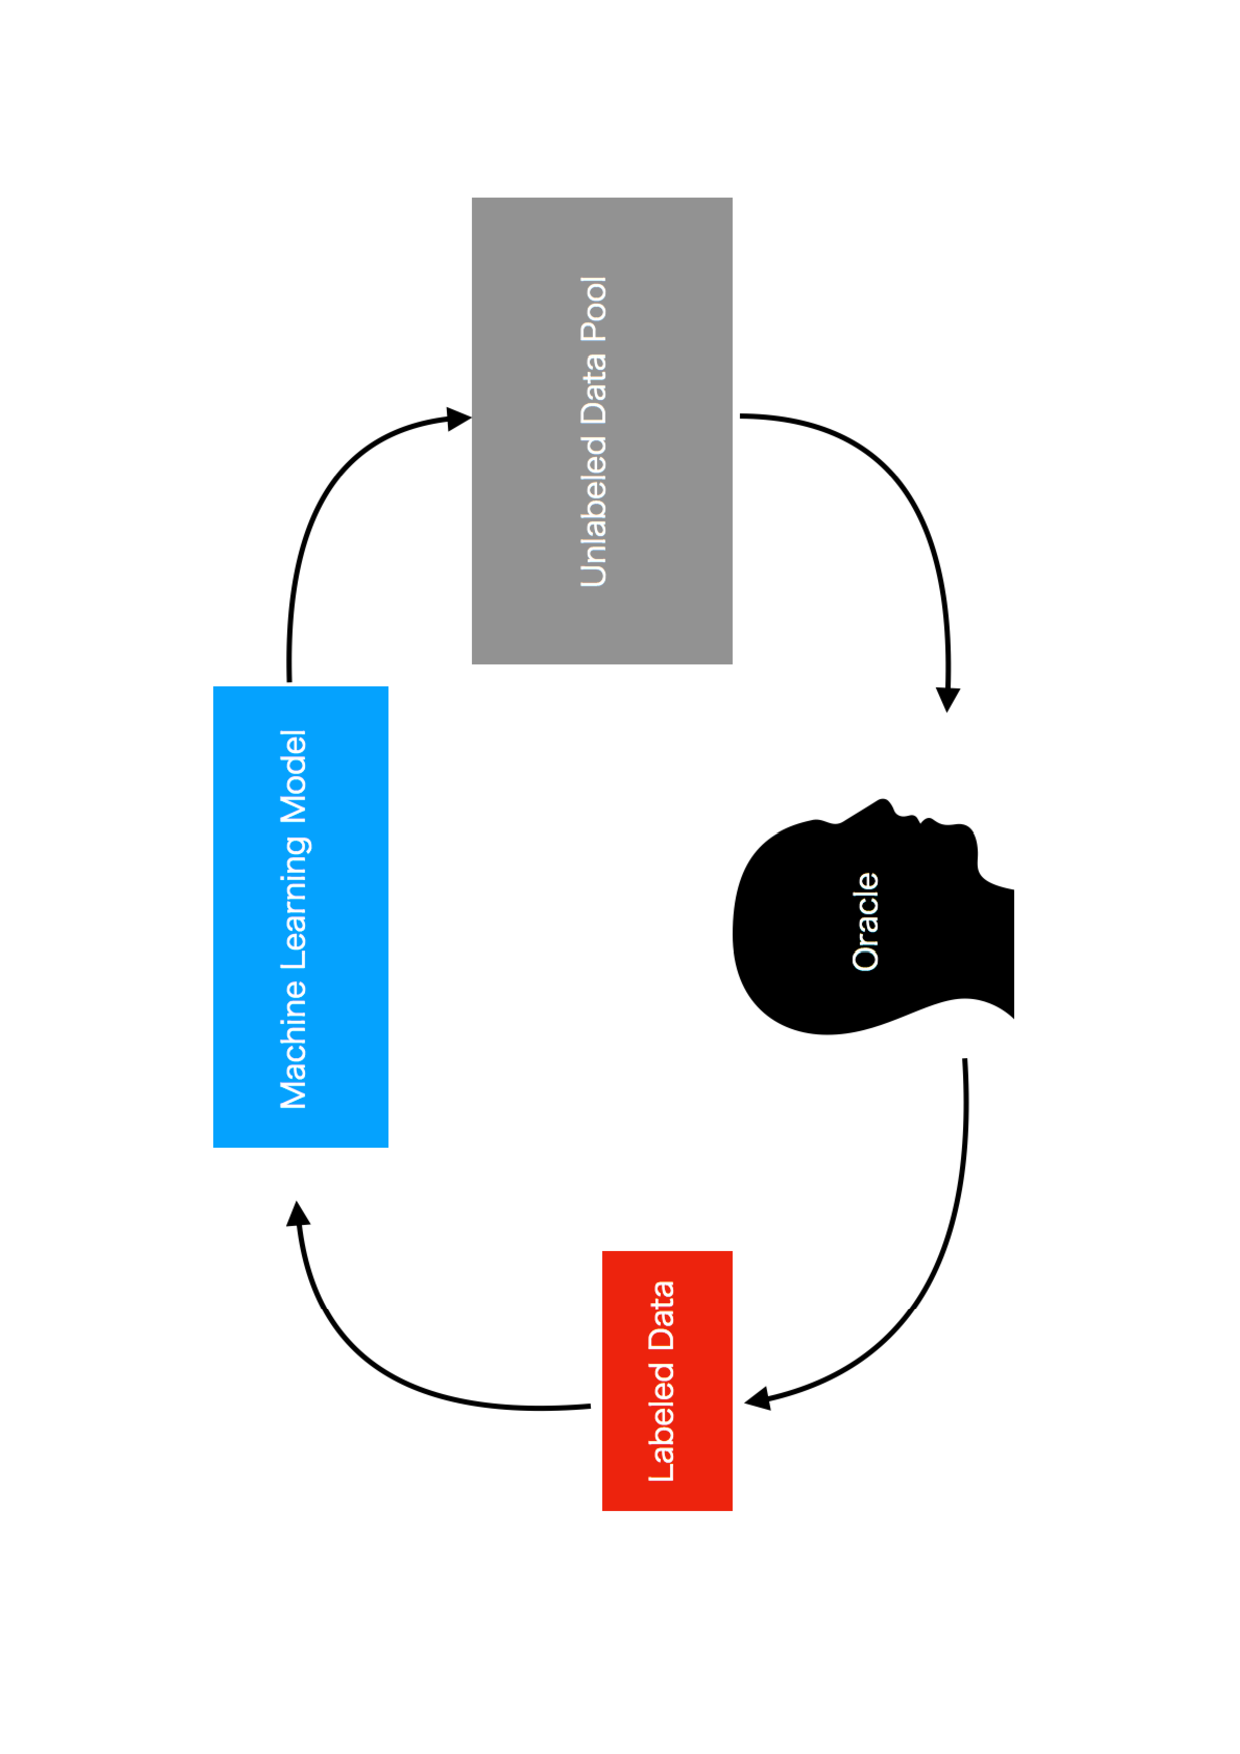
\includegraphics[bb=100 0 470 850, scale=0.4, angle=270]{./images/fig1.pdf}
\vspace{5mm}
\caption{プールベース能動学習の例}
\label{fig1}
\end{center}
\end{figure}

少量のラベル付きデータ集合$L$と大量のラベル無しデータプール$U$が得られると仮定する.
クエリは,この静的なデータプールについて生成する.
典型的には,各インスタンスの情報量尺度の合計がもっとも大きいような部分集合をサンプリングする.

\section{クエリ戦略}
全ての能動学習のシナリオには,各インスタンスの情報量尺度の評価が含まれる.
そのようなクエリ戦略の手法は数多く提案されている.
ここで,$x_A^*$はアルゴリズム$A$によって選択された最も最適なインスタンスとする.

\subsection{Uncertainty Sampling}
最もシンプルなクエリ戦略として,uncertainty samplingが用いられる.
この手法では,学習者はラベル付けの際に最も曖昧であるようなインスタンスについて問い合わせを行う.
例えば,二項分類の確率モデルを用いる場合,事後確率が正である確率が最も0.5に近いようなインスタンスをサンプリングする.
3クラス以上の分類問題においても,以下のように一般化できる.

\begin{equation}
\label{eq1}
    x_{LG}^* = \argmax_{x} \;\; 1 - P_{\theta}(\hat{y}|x)
\end{equation}

ここで$\hat{y}$はモデル$\theta$の下で最も事後確率が高いクラスラベルとなる.
この戦略はシンプルで有効なため,よく用いられている.
しかし,式\ref{eq1}では,最も事後確率の高いクラスに対する曖昧性のみを考慮しており,言い換えると,その他の情報を捨てていることとなる.
これを考慮するため,一部の研究ではmargin samplingと呼ばれる手法を用いる.

\begin{equation}
\label{eq2}
    x_M^* = \argmin_{x} \;\; P_{\theta}(\hat{y_1}|x) - P_{\theta}(\hat{y_2}|x)
\end{equation}

ここで$\hat{y_1}$と$\hat{y_2}$は所与のモデルの元で最も事後確率が高い2つのクラスラベルとなる.
このようにmargin samplingでは2番目に事後確率の高いラベルの情報を組み込んでいる.
直感的に,大きなマージンを持つインスタンスはモデルがラベルの割り当ての際に迷うことが少ないため,自信を持った分類を行うことができると考えられる.
一方で小さなマージンを持つインスタンスは曖昧であることがわかる.
しかし,ラベル集合が大規模である場合には,margin samplingは多くのラベル情報を無視することになる.

より一般的なuncertainty sampling戦略では,不確実性尺度としてエントロピーを用いる.

\begin{equation}
    x_H^* = \argmax_{x} - \sum_{i} P_{\theta}(y_i|x) \log P_{\theta}(y_i|x)
\end{equation}

ここで$y_i$は全ての可能なラベリングの範囲となる.
エントロピーは情報理論的尺度であり,機械学習の文脈において不確実性や不純度などを測る指標として用いられる.

\subsection{Query-By-Committee}
より理論的に動機付けられたクエリ戦略として,query-by-committee (QBC)アルゴリズム\cite{seung1992query}がある.
QBCアルゴリズムは,現在のラベル付きデータ集合から学習されたモデルのcommittee $C = \{\theta^{(1)},\ldots,\theta^{(C)} \}$を維持することを目的とする.
それぞれのcommitteeのメンバはクエリ候補のラベリングに投票できる.
ここで選択すべきインスタンスは,最も投票の割れるようなインスタンスとなる.

不一致度を評価するため,2種類の主要な手法が提案されている.
最初の手法は,エントロピー投票によるものである\cite{dagan1995committee}.

\begin{equation}
    x_{VE}^* = \argmax_{x} - \sum_{i} \frac{V(y_i)}{C} \log \frac{V(y_i)}{C}
\end{equation}

ここで,$y_i$は全てのラベリング可能な範囲にまたがり,$V(y_i)$はcommitteeのメンバの予測による投票数,$C$はcommitteeのサイズとなる.
別の不一致度評価の手法として,Kullback-Leibler (KL) divergenceに基づくものがある\cite{mccallumzy1998employing}.

\begin{equation}
    x_{KL}^* = \argmax_{x} \frac{1}{C} \sum^{C}_{c=1} D(P_{\theta^{(c)}}||P_{C})
\end{equation}

ここで,

\begin{equation}
    D(P_{\theta^{(c)}}||P_{C}) = \sum_{i} P_{\theta^{(c)}}(y_i|x) \log \frac{P_{\theta^{(c)}}(y_i|x)}{P_C(y_i|x)}
\end{equation}

$\theta^{(c)}$はcommittee内の特定のモデルを表現し,$C$はcommittee全体を表す.

\subsection{Expected Model Change}
別の一般的な能動学習フレームワークでは決定論的アプローチを採用しており,ラベルが得られた際に最も現在のモデルに変更を与えるようなインスタンスを選択する.
このようなフレームワークのクエリ戦略の例として,
確率的識別モデルのための''expective gradient length'' (EGL)というアプローチが存在する\cite{settles2008multiple}.

理論的には,EGLは勾配に基づくいかなる学習問題に対しても適用可能である.
確率的識別モデルは通常,勾配に基づいて学習を行うため,モデルに与えられた変化は学習勾配の大きさによって評価できる.
$\nabla l_{\theta}(L)$を目的関数$l$の勾配とする.
ここで,$\nabla l_{\theta}(L \cup \langle x, y\rangle)$は追加でタプル$\langle x, y \rangle$が得られた時の新しい勾配を意味する.
クエリアルゴリズムは事前に真のラベル$y$を知ることはできないので,代わりに可能なラベリングについての勾配の期待値を求める必要がある.

\begin{equation}
    x_{EGL}^* = \argmax_{x} \sum_{i} P_{\theta}(y_i|x) || \nabla l_{\theta}(L \cup \langle x, y_i \rangle)||
\end{equation}

ここで,$||\cdot||$はユークリッドノルムを意味する.
このフレームワークでは,結果のラベルが何であるにせよ,得られるモデルに最も変化をもたらすインスタンスを好むはずであるという仮説に基づく.
このアプローチは経験的実験からうまくいくことが示されている一方で,特徴空間とラベル空間が巨大であるケースでは計算コストが大きくなってしまう.

\subsection{Expected Error Reduction}
その他の決定論的アプローチでは,モデルの変化量ではなく,その汎化誤差の減少量を評価することを目的としている.
そのようなアプローチのうちの一つとして,期待される$0/1$誤差を最小化するものがある.

\begin{equation}
    x_{0/1}^* = \argmin_{x} \sum_{i} P_{\theta}(y_i|x) \left(\sum^U_{u=1} 1 - P_{\theta^{+\langle x, y_i \rangle}}(\hat{y}|x^{(u)})\right)
\end{equation}

ここで$\theta^{+\langle x, y_i \rangle}$はタプル$\langle x, y_i \rangle$がラベル付きデータ集合$L$に追加され,
再学習を行った際の新しいモデルを表す.

多くのケースにおいては,expected error reductionは計算コストの高い手法である.

\section{実用的な考察}
例えば,能動学習の研究においては,その多くがオラクルが単一であり常に正しい結果を返すことを仮定している.
しかし多くの現実の問題において,こうした仮定は成り立たない.
そうした実用問題で考えられる設定に対する研究も近年増えてきている.

\subsection{Batch-Mode Active Learning}
多くの能動学習の研究では,ラベルの問い合わせは連続して,つまり一度に一つのデータのみに対して行われる.
しかしそれでは,全体としての問い合わせ回数が増えてしまうため,モデルの構築には時間がかかってしまう場合がある.
また,アノテーションを行うオラクルが複数人いて,並列にラベル付けを行うことができる場合を考慮すると,シーケンシャルな問い合わせではこれを活かすことができない.
これらの両方のケースを考量すると,連続的な問い合わせは非効率である.
対照的にバッチ型能動学習の手法では,複数のデータをまとめて問い合わせることで,これらの利点を活かすことができる.

バッチ型能動学習は,最適なクエリ集合$Q$を発見することにある.
単純にインスタンスレベルの戦略から$Q-best$クエリを採用することは,情報の重複を考慮しないためうまく動作しないことが多い.
これに対処するために,いくつかのバッチ型能動学習の手法が提案されている\cite{brinker2003incorporating}\cite{guo2008discriminative}\cite{hoi2006batch}.

\subsection{Noisy Oracles}
能動学習のもう一つの強力な仮定のうちの一つに,オラクルによるアノテーションが高品質であるというものがある.
ラベルが経験的実験によるものの場合,その多くは実験環境や計器などの設定によってノイズが含まれる場合が多いはずである.
また,ラベルが人間の専門家によるものだったとしても,それが常に信頼できるものであるとは限らない.
これに対処するような研究も必要となってくる.

\subsection{Variable Labeling Costs}
もし,各インスタンスに対するラベル付与のコストが異なっている場合,能動学習の目的からすれば問い合わせるインスタンス数よりもこのコストを最小化するべきである.
実際のデータセットに対するアノテーションコストについての調査も存在する\cite{settles2008active}.

\begin{itemize}
\item 特定のドメインにおいては,インスタンスごとのアノテーションコストは一定ではなく,大きく異なる場合がある
\item コストを無視した能動学習の手法は,乱択にも劣る場合がある
\item アノテーションのコストは,アノテータによって異なる場合がある
\item アノテーションコストの評価指標には確率的要素が含まれる場合がある
\end{itemize}

\subsection{Multi-Task Active Learning}
典型的な能動学習の設定では,単一のモデルが単一のタスクを解くことを前提としている.
しかし現実の多くの問題では,同じデータは異なる複数の部分タスクのために異なるラベル付けがされる.
Reichartら\cite{reichart2008multi}は2種類のタスクに対する能動学習の手法を提案している.

\subsection{Stopping Criteria}
インタラクティブな学習手法の潜在的な問題の一つに,学習を停止するタイミングについてのものがある.
まず,新しくラベル付けを行うコストが現在のモデルの出力するエラーのコストを上回った時が考えられる.
もう一つの視点として,データの追加による学習精度の向上が頭打ちになったタイミングを観察することが挙げられる.
能動学習は,データ取得のリソースまでを含んだ最適化を目指すため,学習停止の基準を設けることは自然な発想であると言える.

\section{関連分野}

\subsection{Semi-Supervised Learning}
能動学習と同様,半教師あり学習もラベル無しデータを活用することで得られるモデルの性能を向上させることを目的としている.
そのため,これらを組み合わせた研究もいくつか存在する\cite{zhu2003combining}\cite{muslea2002active+}.

\subsection{Submodular Optimization}
劣モジュラ性を持つ関数はいくつかの便利な性質を持つため,これを機械学習分野に適用した研究も多く存在する.
能動学習は部分集合を選択するという問題に一般化でき,応用によっては劣モジュラ最適化問題に落ちる場合もあるため,
これについての研究も存在する\cite{golovin2011adaptive}\cite{golovin2010adaptive}.

\subsection{Graph Structure}
例えばベクトルデータ集合からであれば類似度グラフ,文書集合からであれば共起語グラフの構築などが考えられる.
こうしたラベルの有無によらないデータ集合全体の構造的特性を利用する研究も存在する\cite{jun2016graph}\cite{dasarathy2015s2}.

\bibliographystyle{plain}
\bibliography{reference}
\end{document}
